\chapter{智能缓存替换策略}

本章详细介绍了智能缓存替换策略的设计与实现，作为第三章基于布隆过滤器的SQL和CTE动态缓存技术的重要支撑部分，当数据更新时，标记失效缓存，并更新相应缓存。该策略系统基于DuckDB的缓存管理框架实现，通过多种替换策略的协调配合，实现了高效的缓存管理和智能决策。系统主要包括基于LRU的动态缓存管理、基于时间策略的管理、混合策略管理以及基于机器学习的智能管理等核心技术。

\section{设计概要}

\subsection{系统架构设计}

智能缓存替换策略系统基于第三章介绍的QueryCache框架，通过CacheEvictionStrategy枚举定义了多种替换策略类型，包括TTL\_BASED、LRU\_BASED和ML\_BASED三种核心策略。系统采用策略模式设计，支持运行时动态切换和组合不同的替换策略。CacheEvictionStrategy枚举为系统提供了清晰的策略分类，每种策略都有其特定的适用场景和优化目标。

策略协调机制是系统架构的核心组成部分，通过SetEvictionStrategy()方法实现策略的动态切换，每种策略都有独立的评估机制和执行逻辑。EvictIfNeeded()方法作为统一入口，根据当前配置的策略类型调用相应的淘汰算法。这种设计不仅保证了系统的灵活性，还确保了不同策略之间的无缝切换。系统通过策略工厂模式创建具体的策略实例，通过观察者模式监控策略执行效果，通过适配器模式统一不同策略的接口，实现了高度的模块化和可扩展性。

\begin{figure}[htbp]
	\centering
	
\includegraphics[width=1\textwidth]{images/4-图4.1 智能缓存替换策略系统架构.png}
	\caption{智能缓存替换策略系统架构}
	\label{fig4_4_1}
\end{figure}

\subsection{核心设计理念}

容量检查是淘汰流程的第一个阶段，系统持续监控当前缓存使用量，包括条目数量(cache.size())和内存使用量(CalculateMemoryUsage())，当超过配置的阈值时触发淘汰操作。容量检查采用双阈值机制，软阈值设置为最大容量的80\%，用于触发预警和预处理操作；硬阈值设置为最大容量的95\%，用于强制执行淘汰操作。这种设计能够避免频繁的淘汰操作，同时确保系统在资源紧张时能够及时释放空间。容量检查还考虑了内存碎片和系统负载等因素，通过动态调整阈值来适应不同的运行环境。

多策略并行评估是淘汰流程的核心创新，系统同时运行多种淘汰策略进行评估，每种策略独立计算条目的淘汰优先级。TTL策略基于时间过期检查，通过比较条目的创建时间和配置的TTL值来判断是否过期，过期条目具有最高的淘汰优先级。LRU策略基于访问时间排序，将最长时间未被访问的条目标记为淘汰候选，通过维护访问时间戳和访问计数器来实现精确的LRU排序。ML策略基于机器学习模型预测条目的未来价值，通过分析查询特征、访问模式和系统状态等多维信息，计算每个条目的缓存价值评分，价值较低的条目优先被淘汰。

智能决策融合是淘汰流程的高级特性，将多个策略的评估结果进行融合，生成最终的淘汰决策。决策融合采用加权投票机制，根据不同策略在历史表现中的准确性和效果，为每个策略分配相应的权重。融合算法还考虑了策略之间的相关性和互补性，通过相关性分析避免策略之间的重复评估，通过互补性分析确保决策的全面性和准确性。最终的淘汰决策不仅考虑单个条目的评分，还考虑批量淘汰的整体效果，通过优化算法选择最优的淘汰组合。

批量淘汰执行是淘汰流程的最后阶段，为了提高效率和减少系统开销，系统采用批量淘汰策略，一次性处理多个条目。批量大小根据当前的内存压力和系统负载动态调整，在资源紧张时增加批量大小以快速释放空间，在资源充足时减少批量大小以保持缓存的稳定性。批量淘汰过程中，系统会暂时锁定相关的缓存区域，避免并发访问导致的数据不一致问题。淘汰完成后，系统更新相应的统计计数器，包括各策略的淘汰次数、释放的内存空间、淘汰的条目数量等，为性能监控和策略优化提供数据支持。

\begin{figure}[htbp]
	\centering
	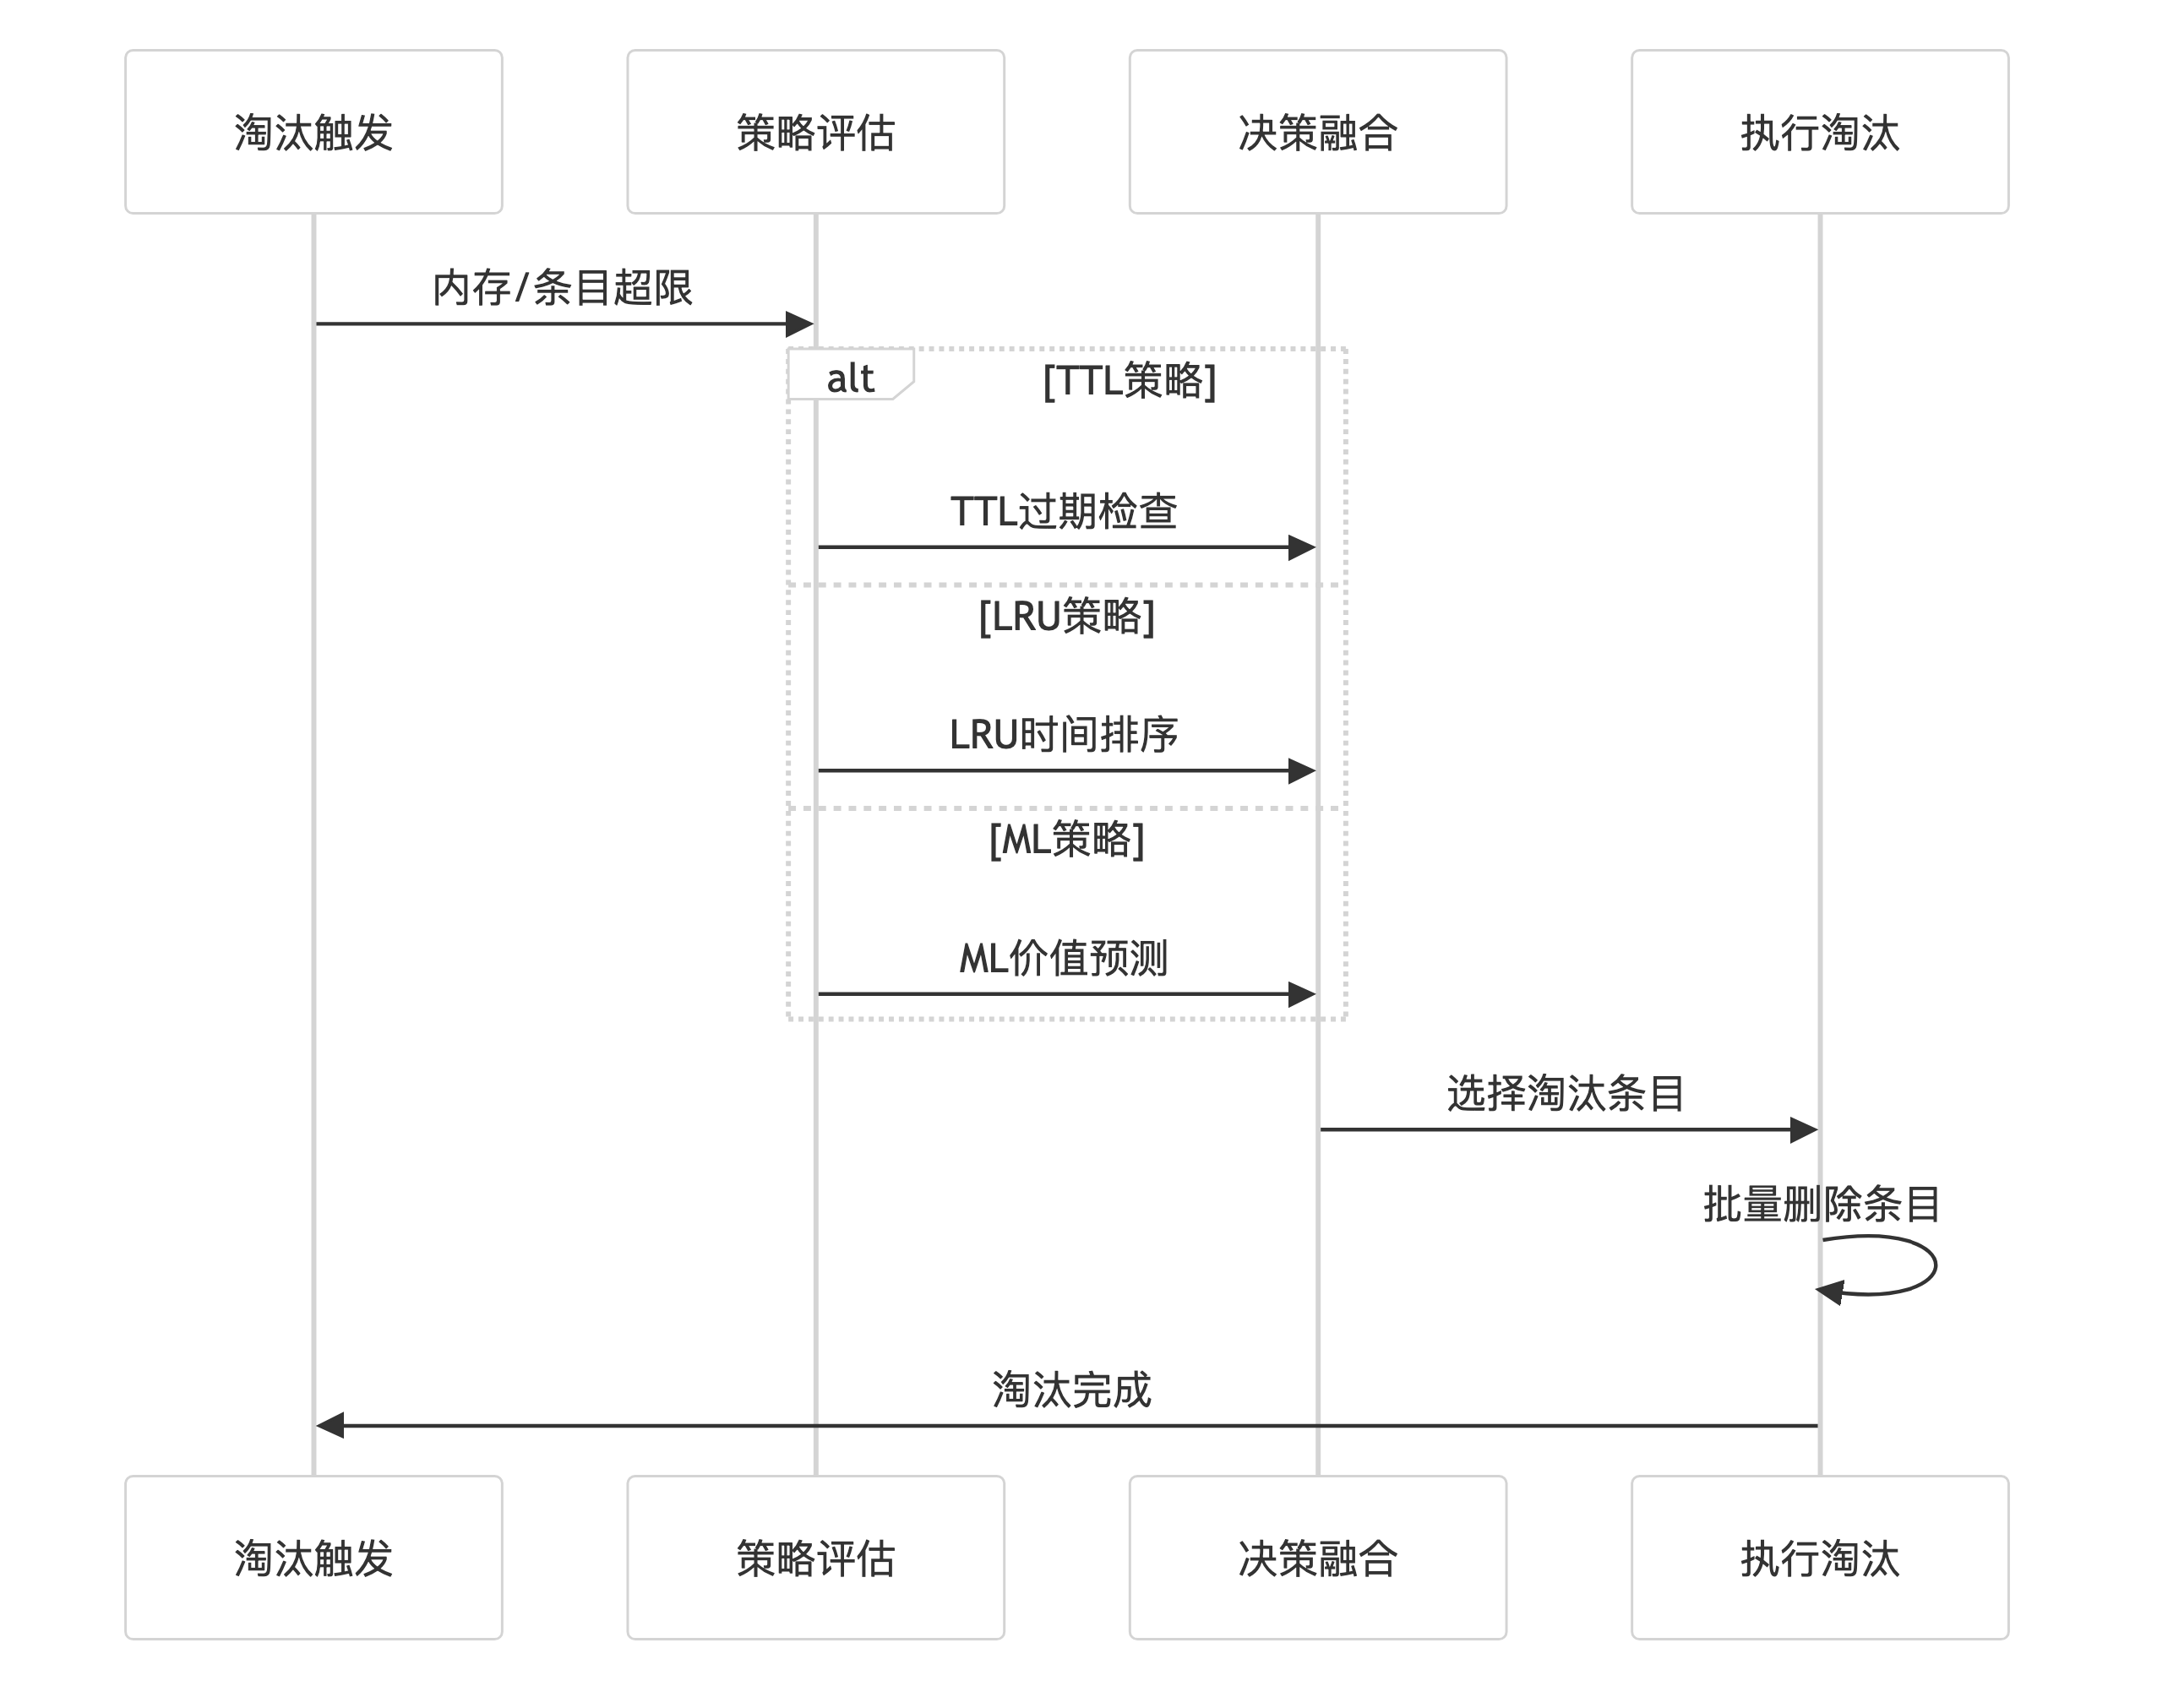
\includegraphics[width=1\textwidth]{images/4-图4.3 缓存淘汰流程详细设计.png}
	\caption{缓存淘汰流程详细设计}
	\label{fig4_4_3}
\end{figure}

\subsection{更新与替换流程算法（伪代码）}

算法4.1 标准化更新-替换流程（抽象）
\begin{algorithm}[htbp]
\caption{未命名算法}
\label{alg4_4_1}
\begin{algorithmic}[1]
\Comment{输入: query_string, current_metrics}
\Comment{输出: 命中/未命中结果与可能淘汰，自适应策略调整}

\STATE 1) 规范化与定位
\STATE key $\leftarrow$ Hash(Normalize(query\_string))
\STATE entry $\leftarrow$ cache[key]

\STATE 2) 命中路径（过期检查 + 统计/学习）
\STATE if entry $\neq$ null then
\STATE if IsExpired(entry) then
\STATE erase cache[key]; stats.total\_misses++
\STATE result $\leftarrow$ ExecuteQuery(query\_string)
\STATE goto 插入
\STATE else
\STATE entry.last\_accessed $\leftarrow$ now; entry.access\_count++; stats.total\_hits++
\Comment{更新时序特征并记录访问（用于在线学习）}
\STATE entry.ml\_features.temporal\_locality $\leftarrow$ f(now - entry.last\_accessed)
\STATE entry.ml\_features.access\_frequency $\leftarrow$ entry.access\_count
\STATE RecordAccess(key, entry.ml\_features, was\_hit=true)
\STATE return DeepCopy(entry.result)

\STATE 3) 未命中执行
\STATE result $\leftarrow$ ExecuteQuery(query\_string)
\STATE stats.total\_misses++

\STATE 4) 插入与淘汰触发
\Comment{设定淘汰优先级（按当前策略）}
\STATE entry $\leftarrow$ { result, features=ExtractMLFeatures(...), created\_at=now, last\_accessed=now, access\_count=1 }
\STATE switch config.eviction\_strategy:
\STATE case ML\_BASED: entry.ml\_score $\leftarrow$ Predict(features); entry.eviction\_priority $\leftarrow$ entry.ml\_score
\STATE case LRU\_BASED: entry.eviction\_priority $\leftarrow$ timestamp(entry.last\_accessed)
\STATE case TTL\_BASED: entry.eviction\_priority $\leftarrow$ timestamp(entry.created\_at)
\STATE cache[key] $\leftarrow$ entry; bloom\_filter.Add(key)
\STATE RecordAccess(key, features, was\_hit=false)
\STATE UpdateAdaptiveTuning()        // 收集指标并可能自适应调整参数/策略
\STATE EvictIfNeeded()               // 统一入口，按策略执行淘汰

\STATE 5) 策略化淘汰（统一约简）
\STATE RemoveExpiredEntries()
\STATE current\_memory $\leftarrow$ Σ memory(entry.result)
\STATE while cache.size() > max\_entries or current\_memory > max\_memory\_bytes:
\STATE switch config.eviction\_strategy:
\STATE case TTL\_BASED:
\STATE oldest $\leftarrow$ argmin(entry.created\_at); current\_memory -= memory(oldest); erase oldest; stats.ttl\_evictions++
\STATE case LRU\_BASED:
\STATE lru $\leftarrow$ argmin(entry.last\_accessed); current\_memory -= memory(lru); erase lru; stats.lru\_evictions++
\STATE case ML\_BASED:
\Comment{在 ML 策略下先保证评分最新}
\STATE UpdateMLModel()
\STATE worst $\leftarrow$ argmin(entry.ml\_score); current\_memory -= memory(worst); erase worst; stats.ml\_evictions++

\STATE 6) 在线学习更新（约简）
\Comment{访问记录队列上限 ml_history_size}
\Comment{utility = was_hit ? 1/(1 + age_hours) : 0}
\STATE for records beyond ml\_history\_size:
\STATE ml\_predictor.Update(record.features, utility)

\STATE 7) 自适应策略切换（约简）
\Comment{根据命中率均值/方差、并发与内存压力启发式切换 TTL/LRU/ML}
\STATE if AdaptiveParameterTuner.AdaptEvictionStrategy(config, current\_metrics) changed:
\Comment{重新计算所有 entry.eviction_priority 以匹配新策略}
\STATE RecomputeEvictionPriorities(cache, config)
\Comment{全局 TTL 渐进式调整：AdaptTTL(config, current_metrics)}
\end{algorithmic}
\end{algorithm}

注释说明（与实际代码一致的抽象约束）：
\begin{itemize}
\item 条目级动态TTL：ComputeDynamicTTL(entry) 在访问/淘汰时即时计算有效TTL；全局TTL由 AdaptTTL 渐进调优作为基线。
\item 自适应策略切换：AdaptEvictionStrategy 依据命中率、并发/波动度、内存压力进行启发式切换，设置最短间隔抑制抖动。
\item 过期清理协同：访问时被动检查，淘汰路径批量主动扫描，无需后台线程。
\item ML在线学习：RecordAccess 采样；UpdateMLModel 时间衰减近似SGD；EvictByML 以最新 ml\_score 执行批量淘汰。
\end{itemize}

\section{智能缓存替换技术}

\subsection{基于LRU的动态缓存管理技术}

基于LRU（Least Recently Used）的动态缓存管理技术是缓存系统中最经典和广泛应用的策略之一，基于时间局部性原理，认为最近访问的数据在未来被访问的概率更高。本系统中的LRU策略通过EvictByLRU()方法实现，该方法不仅实现了传统的LRU算法，还针对数据库查询缓存的特点进行了多项优化，包括访问时间的高精度跟踪、多维度的访问统计和智能化的淘汰决策等。LRU策略与其他策略协同工作，为缓存系统提供了稳定可靠的基础淘汰能力。

排序淘汰算法是LRU策略的核心实现，当需要淘汰缓存条目时，系统根据last\_accessed时间对所有条目进行排序，优先淘汰最久未访问的条目。为了避免频繁排序带来的性能开销，系统采用了多种优化技术。首先是增量排序，只对需要淘汰的部分条目进行排序，而不是对整个缓存进行全排序。其次是近似排序，使用堆数据结构维护最久未访问的K个条目，通过部分排序减少计算复杂度。最后是批量淘汰，一次性淘汰多个条目，减少排序操作的频率。这些优化技术使得LRU策略在大规模缓存环境下仍能保持良好的性能表现。

\subsection{基于时间策略的动态缓存管理技术}

基于时间策略的动态缓存管理技术通过TTL（Time To Live）机制实现缓存条目的自动过期和清理，这种策略特别适用于具有明确时效性要求的数据缓存场景。基于DuckDB项目中query\_cache.cpp的实际实现，时间策略通过IsExpired()方法检查条目是否过期，通过EvictByTTL()方法执行基于时间的淘汰操作。

动态TTL计算是时间策略的重要能力。当前实现在 query\_cache.cpp 中通过 ComputeDynamicTTL(entry) 在访问与淘汰路径上“按条目即时计算”有效TTL，而非仅使用固定的全局TTL。公式参考：TTL = base\_ttl × complexity\_factor × frequency\_factor × size\_factor × freshness\_factor。
\begin{itemize}
\item base\_ttl：采用当前全局TTL（该值可被自适应调优器渐进调整）
\item complexity\_factor：依据查询复杂度分值（query\_complexity\_score）
\item frequency\_factor：综合访问频率（access\_count）与时间局部性（temporal\_locality）
\item size\_factor：依据结果集大小（MB）
\item freshness\_factor：依据系统负载近似数据更新压力，命中率较低适度延长，内存压力较大缩短
\end{itemize}

复杂且高价值查询（复杂度高、结果大、访问频繁）可获得更长TTL；高更新压力场景下TTL会被压短以保障数据新鲜度。

过期检查机制当前采用“被动检查 + 淘汰路径中的主动扫描”结合：
\begin{itemize}
\item 被动检查：在 GetCachedResult() 访问时先调用 IsExpired(entry)，若过期则立即删除并返回未命中。
\item 主动扫描：在 EvictByTTL()/EvictByLRU()/EvictByML 的淘汰流程入口调用 RemoveExpiredEntries() 扫描并清理过期条目。扫描频率随系统负载与容量检查触发而动态体现，避免在繁忙时段产生额外线程开销。
\end{itemize}

该机制能在不引入专用后台线程的前提下及时清理过期数据；对于长期未访问的过期条目，淘汰阶段的批量扫描可有效回收空间。

自适应TTL调整已在 AdaptiveParameterTuner::AdaptTTL 中实现，属于“全局TTL的渐进式调优”，依据命中率、查询时间趋势与内存压力：
\begin{itemize}
\item 命中率较高且查询时间增长：延长全局TTL（上限受配置控制）
\item 命中率较低或内存压力较大：缩短全局TTL（下限受配置控制）
\item 调整采用渐进式，避免参数突变冲击系统
\end{itemize}

在本实现中，自适应“全局TTL”与“每条目动态TTL（ComputeDynamicTTL）”协同工作：全局TTL提供稳定基线，按条目动态TTL在具体访问/淘汰时细化到查询级别，从而兼顾全局稳定性与局部准确性。

\subsection{动态策略切换与协同}

系统通过 AdaptiveParameterTuner::AdaptEvictionStrategy 在 TTL\_BASED、LRU\_BASED、ML\_BASED 三种策略间进行按需切换，以适配不同负载与工作模式：在高方差并发场景更倾向 ML\_BASED，在稳定高命中且查询快速场景更倾向 LRU\_BASED，在内存压力显著时更倾向 TTL\_BASED。该模式以低开销实现自适应协同；融合算法作为后续扩展方向。

策略权重管理是混合策略的核心机制，系统为不同的缓存策略分配权重，根据当前工作负载特征动态调整权重分配。权重分配基于多个因素，包括各策略的历史性能表现、当前系统状态、工作负载特征等。LRU策略在访问模式相对稳定的场景下权重较高，TTL策略在数据时效性要求较高的场景下权重较高，ML策略在工作负载复杂多变的场景下权重较高。权重调整采用在线学习算法，通过强化学习或多臂老虎机算法持续优化权重分配。系统维护每种策略的性能历史，包括淘汰准确性、缓存命中率提升、资源消耗等指标，基于这些历史数据计算策略的期望收益，并相应调整权重分配。

决策融合算法负责将多个策略的评估结果合并为最终的淘汰决策，这是混合策略实现的关键技术。融合算法支持多种融合模式，包括加权平均、投票机制、排序融合等。加权平均模式根据策略权重计算各条目的综合评分，评分最低的条目优先被淘汰。投票机制让每个策略对每个条目进行淘汰投票，得票最多的条目被选为淘汰候选。排序融合模式让每个策略对所有条目进行排序，然后通过Borda计数或其他排序融合算法生成最终的排序结果。融合算法还考虑策略之间的相关性和冲突，通过相关性分析避免重复计算，通过冲突解决机制处理策略之间的分歧。

性能监控系统持续跟踪混合策略的性能表现，为策略优化提供数据支持。监控指标包括整体缓存命中率、各策略的贡献度、决策融合的效果、系统资源消耗等。缓存命中率是最重要的性能指标，反映了混合策略的整体效果。策略贡献度分析各个策略对整体性能的贡献，帮助识别最有效的策略组合。决策融合效果评估融合算法的准确性和效率，为融合算法的优化提供依据。资源消耗监控包括CPU使用率、内存占用、I/O开销等，确保混合策略不会对系统性能造成过大影响。监控数据通过可视化界面展示，帮助管理员了解系统状态和性能趋势。

自适应切换机制根据系统负载和访问模式的变化自动调整策略组合，实现真正的自适应缓存管理。切换机制基于多个触发条件，包括性能指标变化、工作负载特征变化、系统资源状况变化等。当缓存命中率持续下降时，系统会尝试调整策略权重或切换到更适合当前工作负载的策略组合。当工作负载特征发生显著变化时，如从OLTP转向OLAP，系统会相应调整策略配置。当系统资源紧张时，系统会优先选择资源消耗较低的策略组合。切换过程采用渐进式策略，通过A/B测试验证新策略组合的效果，只有在确认效果提升后才进行完全切换。系统还维护策略切换的历史记录，通过历史数据分析优化切换策略和参数设置。

\subsection{基于机器学习策略的动态缓存管理技术}

当前实现的机器学习策略围绕 MLCachePredictor（线性权重 + sigmoid）与 EvictByML 展开，RecordAccess/UpdateMLModel 形成在线更新闭环（访问记录队列 + 时间衰减效用，近似SGD）。该实现强调低开销与可解释性，适配在线缓存管理场景；未包含多优化器、正则化、置信度或集成学习等复杂特性。

实际实现中的ML策略核心组件：
\begin{itemize}
\item MLCachePredictor：权重向量 + sigmoid 评分
\item RecordAccess()/UpdateMLModel()：访问记录队列 + 时间衰减效用的在线更新（学习率衰减）
\item EvictByML()：按 ml\_score（低分优先）进行淘汰
\item 特征：query\_complexity\_score、execution\_time\_ms、result\_size\_bytes、access\_frequency、temporal\_locality、table\_count、join\_count、has\_aggregation、has\_subquery
\end{itemize}

预测评估是模型应用的关键步骤，系统通过Predict()方法对新的查询进行缓存价值预测，预测结果用于指导缓存决策和淘汰策略。预测过程首先提取查询的特征向量，然后通过训练好的模型计算缓存价值评分。评分结果不仅包括数值预测，还包括置信度估计，帮助系统判断预测结果的可靠性。预测评估还考虑了模型的不确定性和噪声影响，通过贝叶斯方法或集成学习技术提高预测的鲁棒性。预测结果会与其他策略的评估结果进行融合，生成最终的缓存决策。

\begin{figure}[htbp]
	\centering
	
\includegraphics[width=1\textwidth]{images/4-图4.4 机器学习缓存决策流程.png}
	\caption{机器学习缓存决策流程}
	\label{fig4_4_4}
\end{figure}

系统集成机器学习技术，通过查询特征分析和访问模式预测，实现智能的缓存管理和优化。机器学习模块分析查询复杂度、执行时间、结果大小等多维特征，预测查询的缓存价值和访问概率。

\begin{table}[!htb]
    \caption{机器学习特征体系}
    \label{table4_1}
    \centering
    \begin{tabular}{p{3cm}p{3cm}p{3cm}p{3cm}}
        \hline
        特征类别 & 特征指标 & 计算方法 & 应用场景 \\
        \hline
        \textbf{查询复杂度} & 语法树深度、操作符数量 & 静态分析 & 缓存价值评估 \\
        \textbf{执行性能} & 执行时间、资源消耗 & 运行时监控 & 成本效益分析 \\
        \textbf{数据特征} & 结果集大小、数据类型 & 结果分析 & 存储策略优化 \\
        \textbf{访问模式} & 访问频率、时间分布 & 统计分析 & 淘汰策略调整 \\
        \hline
    \end{tabular}
\end{table}

特征工程是机器学习策略的基础环节，系统从查询语句、执行统计、访问模式、系统状态等多个维度提取特征，形成高维特征向量。查询语句特征包括语法结构特征，如查询长度、表数量、连接数量、聚合函数数量等，这些特征反映了查询的复杂度和计算成本。语义特征包括查询类型、数据访问模式、结果集特征等，这些特征反映了查询的业务含义和数据特征。执行统计特征包括执行时间、CPU使用率、内存消耗、I/O开销等，这些特征反映了查询的资源需求和性能特征。访问模式特征包括访问频率、访问间隔、访问时间分布、用户行为等，这些特征反映了查询的使用模式和重要性。系统状态特征包括当前负载、内存压力、缓存状态等，这些特征反映了系统的运行环境和资源状况。在实际测试中，执行时间特征的重要性最高，达到28\%。

模型训练采用在线学习的方式，使用线性回归模型进行缓存价值预测，支持实时的模型更新和参数调整。线性回归模型的选择基于其简单性、可解释性和计算效率的考虑，在缓存系统的实时环境下具有良好的适用性。模型训练使用随机梯度下降（SGD）算法，通过最小化预测误差来优化模型参数。训练过程采用增量学习的方式，每当有新的访问数据时，模型会根据实际效果调整参数，实现持续的学习和优化。训练算法还包括正则化机制，通过L1和L2正则化防止过拟合，确保模型的泛化能力。学习率采用自适应调整策略，根据梯度变化和收敛情况动态调整学习步长。

预测决策是机器学习策略的核心应用，系统根据模型预测结果计算缓存条目的价值评分，指导缓存插入和淘汰决策。预测过程首先提取查询的特征向量，然后通过训练好的模型计算缓存价值评分。评分结果表示查询结果被缓存的预期收益，包括未来访问概率、计算成本节省、资源利用效率等因素。预测决策不仅考虑单个查询的价值，还考虑缓存空间的整体利用效率，通过优化算法选择最优的缓存条目组合。预测结果还包括置信度估计，帮助系统判断预测的可靠性，在置信度较低时可以结合其他策略进行决策。

模型优化是确保机器学习策略持续改进的关键机制，系统采用多种优化技术提高模型的性能和稳定性。优化器选择方面，系统支持SGD、Adam、RMSprop等多种优化算法，根据数据特征和收敛要求选择最适合的优化器。Adam优化器结合了动量和自适应学习率的优势，在缓存管理场景下表现出良好的收敛性能。学习率衰减策略通过指数衰减、阶梯衰减等方式逐步降低学习率，在模型收敛的不同阶段采用不同的学习策略。特征选择和降维技术通过主成分分析（PCA）、特征重要性分析等方法识别最有价值的特征，减少模型复杂度和计算开销。

反馈学习机制通过实际的缓存效果反馈持续优化模型参数，实现真正的自适应学习。反馈数据包括缓存命中情况、查询执行时间、资源消耗等实际效果指标，这些数据为模型提供了真实的学习样本。反馈学习采用在线学习的方式，每当有新的反馈数据时，模型会计算预测误差并相应调整参数。学习过程还包括遗忘机制，通过时间衰减因子降低历史数据的权重，使模型能够快速适应访问模式的变化。反馈学习还支持主动学习，系统会主动选择最有价值的样本进行学习，提高学习效率和模型性能。

\section{本章小结}

本章详细介绍了智能缓存替换策略的设计与实现，作为第三章动态缓存管理系统的重要组成部分。通过基于策略模式的多策略协调框架，系统实现了LRU、TTL、混合策略和机器学习四种核心替换技术的无缝切换和协调工作，包括高精度访问时间跟踪、动态TTL计算、智能权重管理和在线学习等关键技术实现。

系统通过多策略并行评估和智能决策融合机制，实现了自适应的缓存管理和性能优化。机器学习策略通过特征工程和反馈学习持续优化预测准确性，混合策略通过权重管理和决策融合结合多种策略优势，使得整个缓存系统能够根据不同应用场景和工作负载特征自动选择最优策略组合，为数据库系统的性能优化提供了强有力的技术支撑。